\documentclass{report}

% Paquetes y configuraciones adicionales
\usepackage{graphicx}
\usepackage[export]{adjustbox}
\usepackage{caption}
\usepackage{float}
\usepackage{titlesec}
\usepackage{geometry}
\usepackage[hidelinks]{hyperref}
\usepackage{titling}
\usepackage{titlesec}
\usepackage{parskip}
\usepackage{wasysym}
\usepackage{tikzsymbols}
\usepackage[spanish]{babel}

\newcommand{\subtitle}[1]{
  \posttitle{
    \par\end{center}
    \begin{center}\large#1\end{center}
    \vskip0.5em}
}

% Configura los márgenes
\geometry{
    left=2cm,   % Ajusta este valor al margen izquierdo deseado
    right=2cm,  % Ajusta este valor al margen derecho deseado
    top=3cm,
    bottom=3cm,
}

% Configuración de los títulos de las secciones
\titlespacing{\section}{0pt}{\parskip}{\parskip}
\titlespacing{\subsection}{0pt}{\parskip}{\parskip}
\titlespacing{\subsubsection}{0pt}{\parskip}{\parskip}

% Redefinir el formato de los capítulos y añadir un punto después del número
\makeatletter
\renewcommand{\@makechapterhead}[1]{%
  \vspace*{0\p@} % Ajusta este valor para el espaciado deseado antes del título del capítulo
  {\parindent \z@ \raggedright \normalfont
    \ifnum \c@secnumdepth >\m@ne
        \huge\bfseries \thechapter.\ % Añade un punto después del número
    \fi
    \interlinepenalty\@M
    #1\par\nobreak
    \vspace{10pt} % Ajusta este valor para el espacio deseado después del título del capítulo
  }}
\makeatother

\makeatletter
\renewcommand\chapter{\@startsection{chapter}{0}{\z@}%
    {-3.5ex \@plus -1ex \@minus -.2ex}%
    {2.3ex \@plus.2ex}%
    {\normalfont\Large\bfseries}}
\makeatother

\begin{document}

% Portada del informe

\title{Práctica 04. Disparadores y Vistas en SQL}
\subtitle{Administracion y Diseño de Bases de Datos}
\author{Cheuk Kelly Ng Pante}
\date{\today}

\maketitle

% Índice
\tableofcontents

% Nueva página para el primer capítulo
\cleardoublepage

% Secciones del informe
% Capitulo 1
\chapter{Realizar la restauración de la base de datos alquiler.tar}
Para realizar la restauración de la base de datos \emph{alquiler.tar}, primero debemos crear la base de datos \emph{ALQUILERDVD} y luego restaurar la base de datos con el comando \emph{pg\_restore}, como se muestra a continuación:
\begin{verbatim}
usuario@ubuntu# pg_restore -U postgres -d alquilerdvd ./alquiler.tar
\end{verbatim}

\begin{figure}[H]
  \centering
  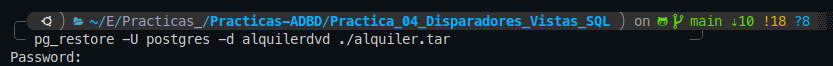
\includegraphics[scale=0.55]{img/restore_DB.png}
  \caption{Restauración de la base de datos}
  \label{fig:restauración de la base de datos}
\end{figure}

% Capitulo 2
\chapter{Identificacion de las tablas, vistas y secuencias}
Para identificar las tablas, vistas y secuencias de la base de datos \emph{ALQUILERDVD}, hay que usar la terminal interactiva de \emph{PostgreSQL} y ejecutar los siguiente comandos:
\begin{verbatim}
usuario@ubuntu# sudo -u postgres psql
postgres=# \c alquilerdvd 
alquilerdvd=# \dt
alquilerdvd=# \dv
alquilerdvd=# \ds
\end{verbatim}

\begin{figure}[H]
  \centering
  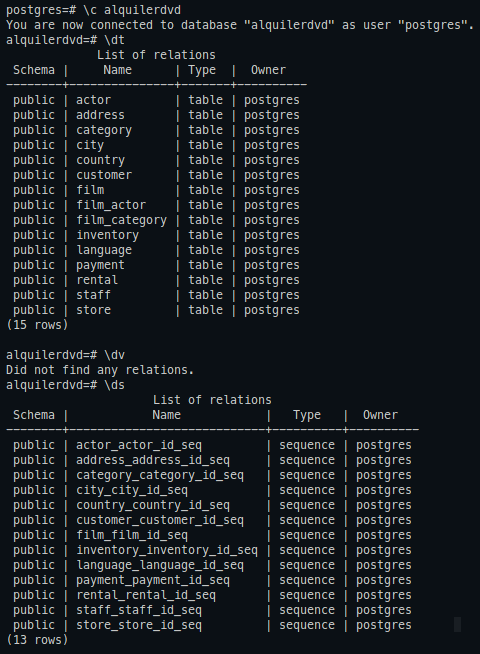
\includegraphics[scale=0.48]{img/tablas_vistas_secuencias.png}
  \caption{Identificación de las tablas, vistas y secuencias}
  \label{fig:identificación de las tablas, vistas y secuencias}
\end{figure}

% Capitulo 3
\chapter{Identifique las tablas principales y sus principales elementos}

% Tabla: actor
\CIRCLE \ \ \textbf{Tabla:} \emph{actor}
\begin{itemize}
  \item \textbf{Descripción:} Contiene la información de los actores.
  \item \textbf{Elementos:} \emph{actor\_id, first\_name, last\_name, last\_update}
\end{itemize}

% Tabla: address
\CIRCLE \ \ \textbf{Tabla:} \emph{address}
\begin{itemize}
  \item \textbf{Descripción:} Contiene la información de las direcciones.
  \item \textbf{Elementos:} \emph{address\_id, address, address2, district, city\_id, postal\_code, phone, last\_update}
\end{itemize}

% Tabla: category
\CIRCLE \ \ \textbf{Tabla:} \emph{category}
\begin{itemize}
  \item \textbf{Descripción:} Contiene la información de las categorías.
  \item \textbf{Elementos:} \emph{category\_id, name, last\_update}
\end{itemize}

% Tabla: city
\CIRCLE \ \ \textbf{Tabla:} \emph{city}
\begin{itemize}
  \item \textbf{Descripción:} Contiene la información de las ciudades.
  \item \textbf{Elementos:} \emph{city\_id, city, country\_id, last\_update}
\end{itemize}

% Tabla: country


\end{document}